% Created 2023-08-28 月 13:11
% Intended LaTeX compiler: pdflatex
\documentclass[10pt]{article}
\usepackage[utf8]{inputenc}
\usepackage[T1]{fontenc}
\usepackage{graphicx}
\usepackage{longtable}
\usepackage{wrapfig}
\usepackage{rotating}
\usepackage[normalem]{ulem}
\usepackage{amsmath}
\usepackage{amssymb}
\usepackage{capt-of}
\usepackage{hyperref}
\usepackage[newfloat]{minted}
\usepackage[a4paper, total={6.5in, 9in}]{geometry}
\usepackage{minted}
\setminted{breaklines}
\usepackage[utf8]{inputenc}
\renewcommand{\familydefault}{\sfdefault}
\usemintedstyle{vs}
\usepackage[most]{tcolorbox}
\usepackage{CJKutf8}
\usepackage{xurl}
\usepackage{fontawesome5}
\usepackage{hyperref}
\usepackage{graphicx}
\usepackage{float}
\newcommand{\gitlab}[1]{%
\href{#1}{GitLab \faGitlab}}
\author{Vincent Conus}
\date{2023-8-24}
\title{Setting up and using Xilinx KRIA KV260\\\medskip
\large \begin{CJK}{UTF8}{min}南山大学\end{CJK}}
\hypersetup{
 pdfauthor={Vincent Conus},
 pdftitle={Setting up and using Xilinx KRIA KV260},
 pdfkeywords={},
 pdfsubject={A report presenting how to use and set Xilinx's Kria board},
 pdfcreator={Emacs 30.0.50 (Org mode 9.6.6)}, 
 pdflang={English}}
\begin{document}

\begin{titlepage}
\centering
{\LARGE Setting up and using Xilinx KRIA KV260 \par }
\vspace{5mm}
{\large \begin{CJK}{UTF8}{min}南山大学\end{CJK} \par}
\vspace{1cm}
{\large 2023-8-24 \par}
\vspace{2cm}
{\large Vincent Conus -  Source available at \gitlab{https://gitlab.com/sunoc/xilinx-kria-kv260-documentation} \par}
\vspace{3cm}
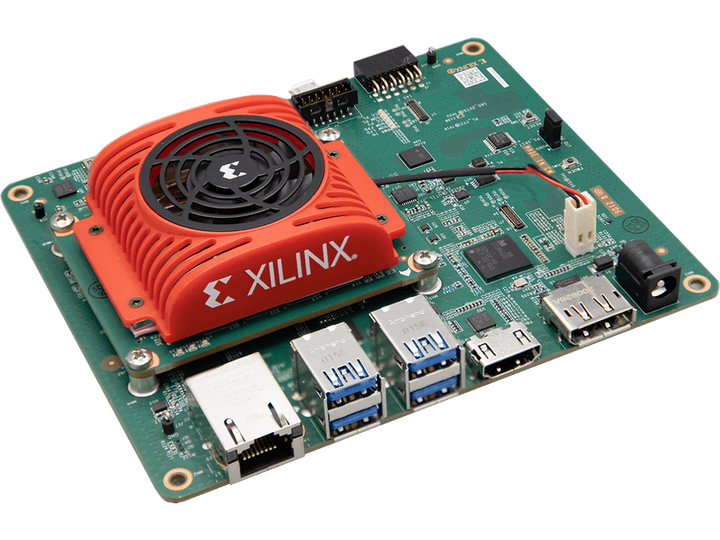
\includegraphics[width=0.8\textwidth]{./img/board}\end{titlepage}
\tableofcontents
\pagebreak
\section{Introduction}
\label{sec:orgf97e357}

\subsection{Motivation}
\label{sec:orgae777db}
This guide will present how to setup and use Xilinx's KRIA board, in particular
for running ROS on a host Ubuntu system, as well as for deploying
micro-ROS as a firmware on the MCU part of this board's chip.

The use of this device in particular is interesting because of the presence
of a CPU comprising both a general purpose ARM core, capable of running
a Linux distribution, as well as another ARM core, real-time enabled,
capable to run a RTOS.

\subsection{Build instructions for this report}
\label{sec:org0f400d4}
The base file for this report is actually this README.org file itself.
However, upon local build, this file is regularly exported as
a \texttt{.tex} file that can be built normally.
On a moderately recent Ubuntu-base distribution, the following packages seemed to be required to build the
report:

\begin{minted}[frame=single,framesep=2mm,baselinestretch=1.2,linenos,breaklines,fontsize=\footnotesize]{bash}
sudo apt-get install texlive-base texlive-latex-recommended texlive-lang-japanese
\end{minted}

Then, the actual build can be made with a simple:

\begin{minted}[frame=single,framesep=2mm,baselinestretch=1.2,linenos,breaklines,fontsize=\footnotesize]{bash}
pdflatex README.tex
\end{minted}

No fancy Lua or theme at the moment !

\subsubsection{Automatic build with CI/CD pipeline}
\label{sec:orgbb6d28c}
If you don't want to build the report yourself, a CI pipeline is used to make it on GitLab.

You can check the steps in the .gitlab-ci.yml file.
This build uses a base Ubuntu image and basically takes the same steps as presented above for a local build.

A PDF artifact can be downloaded.

\subsubsection{Headers and \LaTeX{} settings for export}
\label{sec:org1a4f29d}
A large amount of headers and parameters are needed in order
to have this "README" document being exportable as a \LaTeX{}
document formatted the way I wanted it to be.

The detail can be seen in the raw \texttt{.org} version of this README.

\section{Boot firmware}
\label{sec:orgea33363}
The goal for the Linux side of the deployment is to
have the latest LTS version of Ubuntu up and running.
In order to be able to boot such a newer version of Linux, the
boot image of the board must first be updated.

The procedure is available in \href{https://docs.xilinx.com/r/en-US/ug1089-kv260-starter-kit/Firmware-Update}{the official documentation},
but I will present it step by step here.

\subsection{Getting the new firmware}
\label{sec:org00affa0}
A 2022 version of the board firmware is required in order to run the latest
version of Ubuntu properly.

The image can be downloaded at \href{https://xilinx-wiki.atlassian.net/wiki/spaces/A/pages/1641152513/Kria+K26+ SOMoot-FW-update-with-xmutil}{the atlassian page} on the topic,
or even directly with the following command:

\begin{minted}[frame=single,framesep=2mm,baselinestretch=1.2,linenos,breaklines,fontsize=\footnotesize]{sh}
wget https://www.xilinx.com/member/forms/download/\
     design-license-xef.html?filename=BOOT-k26-starter-kit-20230516185703.bin
\end{minted}


\subsection{Reaching the board recovery tool}
\label{sec:org0139d77}
Now the firmware \texttt{.bin} image is available, it is possible to update it using the
boards recovery tool. Here are the steps that must be taken in order to reach
this tool and update the board:

\begin{itemize}
\item Connect the board to your machine via a Ethernet cable.
This will obviously cut you internet access, so you should be set for that.
\item Select the wired network as your connection (must be "forced", since it
doesn't have internet access).
\item Set a fixed IP address for your machine, in the \texttt{192.168.0.1/24}
range, except the specific \texttt{192.168.0.111}, which will be used by the
board.
\item Using a web browser on your host machine, access
\texttt{http://192.168.0.111}. Thou shall now see the interface, as visible on
the figure \ref{fig:orgd34b983} below.
\end{itemize}

\begin{figure}[htbp]
\centering
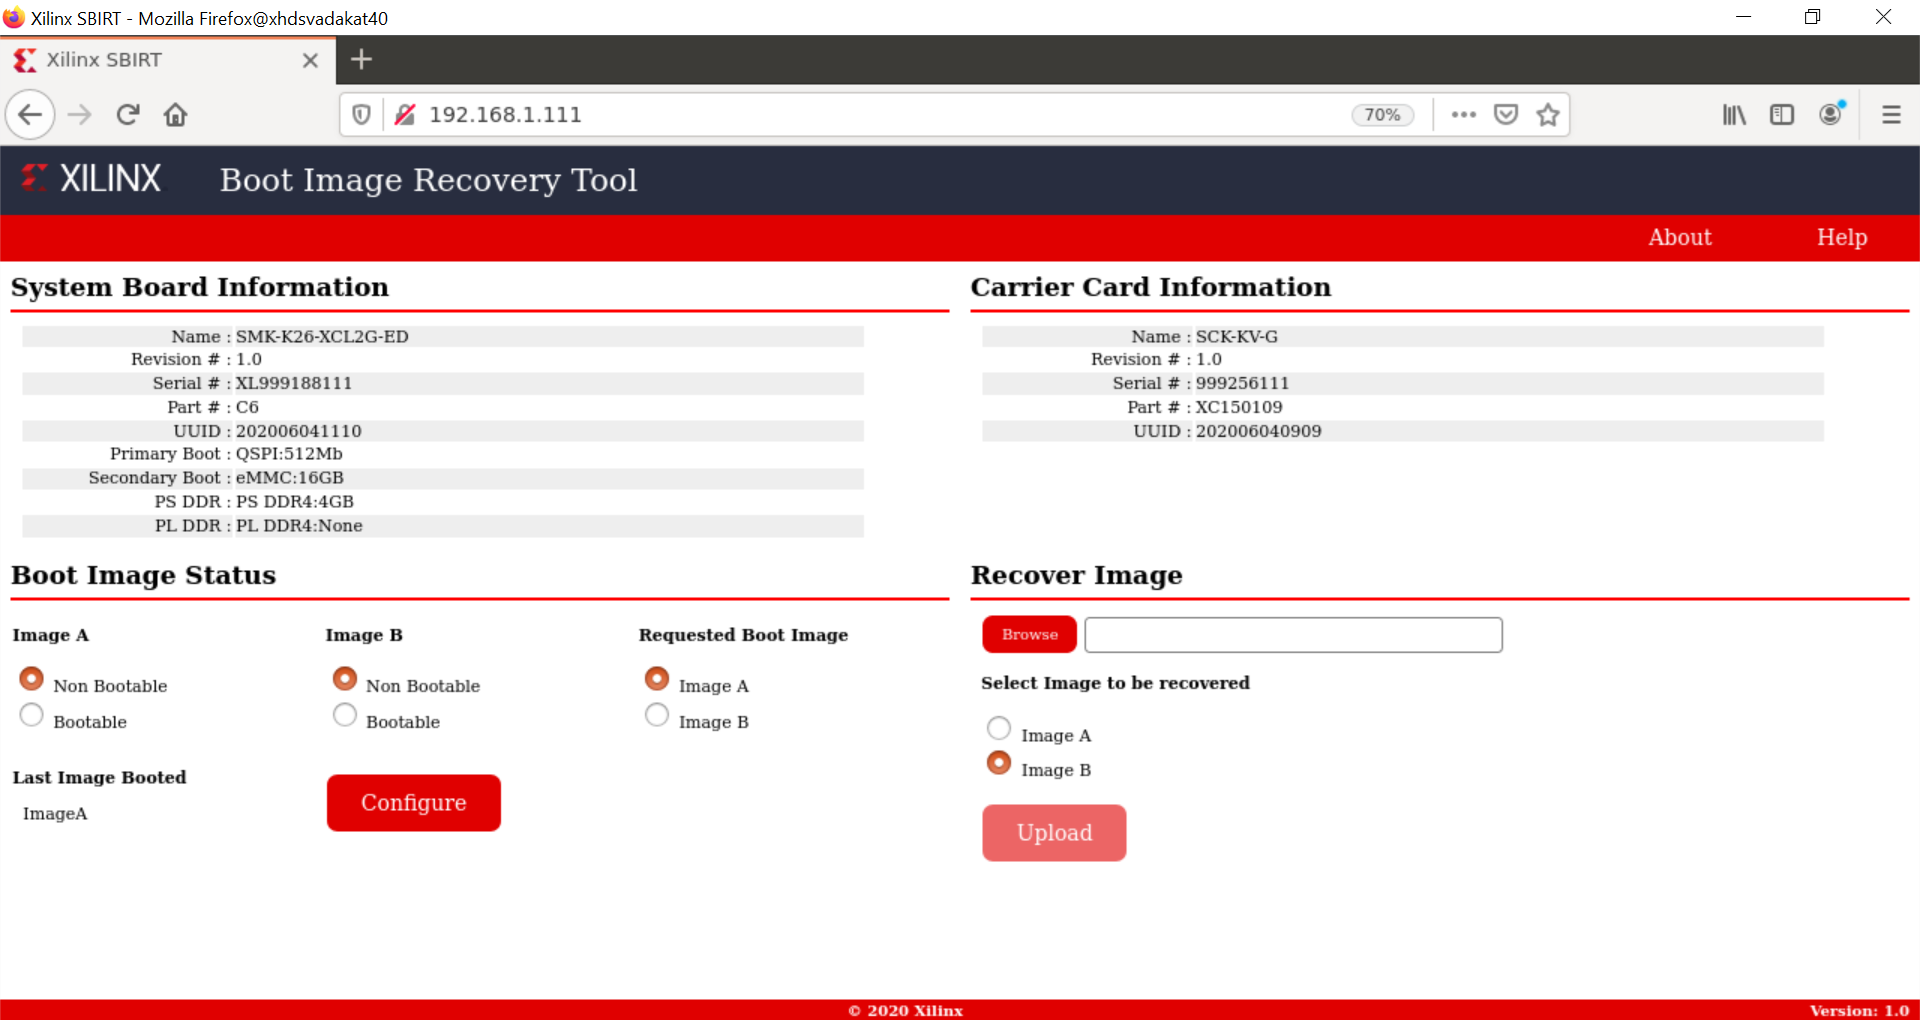
\includegraphics[width=1\textwidth]{img/recovery.png}
\caption{\label{fig:orgd34b983}The recovery tool for the board, access from Firefox. We can see board information at the center, and the tools to upload the firmware at the bottom of the page.}
\end{figure}

\subsection{Updating the boot firmware}
\label{sec:org163c07f}
From this "recovery" page, it is possible to upload the \texttt{.bin} file downloaded previously onto
the board using the "Recover Image" section at the bottom right of the page.

The board can be re-booted afterwards.

\section{Installing Linux}
\label{sec:org680a92b}
Withe the boot firmware being up-to-date, we can proceed to install a Linux distribution
on our Kria board. The step needed to archive a full installation of Ubuntu 22.04
will be presented in this section.

\subsection{Preparing and booting a Ubuntu 22.04 media}
\label{sec:org14f39e4}
An \href{https://ubuntu.com/download/amd-xilinx}{official Ubuntu image} exists and is
provided by Xilinx, allowing the OS installation to be quick and
straightforward.
Ubuntu is a common and easy to use distribution. Furthermore,
it allows to install ROS2 as a package, which is most convenient and will be
done later in this guide.

Once the image has been downloaded at \href{https://ubuntu.com/download/amd-xilinx}{Canonical's page}
we can flash it onto the SD card, with the following instructions.

\begin{tcolorbox}[colback=red!5!white,colframe=red!75!black]
\textbf{DANGER}: The next part involve the \texttt{dd} command writing on disks!!!
As always with the dd command, thou have to be \textbf{VERY} careful on what arguments
thou give. Selecting the wrong disk will result on the destruction of
thy data !!
\uline{If you are unsure of what to do, seek assistance !}
\end{tcolorbox}

With the image available on thy machine and a SD card visible as \texttt{/dev/sda}
Once the SD card is flashed and put back in the board, the micro-USB cable can be
connected from the PC to the board. It is then possible to
connect to the board in serial with an appropriate tool, for example \texttt{picocom},
as in the following example (the serial port that "appeared" was the \texttt{/dev/ttyUSB1} in this case,
and the 115200 bitrate is the default value for the board):

\begin{minted}[frame=single,framesep=2mm,baselinestretch=1.2,linenos,breaklines,fontsize=\footnotesize]{sh}
sudo picocom /dev/ttyUSB1 -b 115200
\end{minted}

Once logged in, it is typically easier and more convenient to connect the board
using SSH. When the board is connected to the network, it is possible to know
it's IP address with the \texttt{ip} command; then it is possible to connect to
the board with ssh, as follow (example, with the first command to be run on the board
and the second one on the host PC, both without the first placeholder hostnames):


\begin{minted}[frame=single,framesep=2mm,baselinestretch=1.2,linenos,breaklines,fontsize=\footnotesize]{sh}
kria# ip addr

host# ssh ubuntu@192.168.4.11
\end{minted}

\subsection{Network and admin setups}
\label{sec:org6f47199}
This section presents a variety of extra convenience configurations
that can be used when setting-up the Kria board.

\subsubsection{Proxy and DNS}
\label{sec:org96776b1}
An issue that can occur when connecting the board to the internet is the
conflicting situation with the university proxy.
Indeed, as the network at Nanzan University requires to go through a proxy,
some DNS errors appeared.

Firstly, it is possible to set a DNS IP address in \texttt{/etc/resolv.conf} by
editing it and adding your favorite DNS, for example \texttt{nameserver 1.1.1.1}
next to the other \texttt{nameserver} entry. The resolver can then be restarted.

\begin{minted}[frame=single,framesep=2mm,baselinestretch=1.2,linenos,breaklines,fontsize=\footnotesize]{sh}
sudo nano /etc/resolv.conf

sudo systemctl restart systemd-resolved
\end{minted}

Secondly, it might become needed to setup the proxy for the school.

This can be done as follow, by exporting a https base proxy configuration
containing you AXIA credentials (this is specific to Nanzan University IT system),
then by consolidating the configuration for other types of connections in the \texttt{bashrc}:

\begin{minted}[frame=single,framesep=2mm,baselinestretch=1.2,linenos,breaklines,fontsize=\footnotesize]{sh}
export https_proxy="http://<AXIA_username>:\
       <AXIA_psw>@proxy.ic.nanzan-u.ac.jp:8080"

echo "export http_proxy=\""$https_proxy"\"" >> ~/.bashrc \
     echo "export https_proxy=\""$https_proxy"\"" >> ~/.bashrc \
     echo "export ftp_proxy=\""$https_proxy"\"" >> ~/.bashrc \
     echo "export no_proxy=\"localhost, 127.0.0.1,::1\"" \
     >> ~/.bashrc
\end{minted}

Eventually the board can be rebooted in order for the setup to get applied cleanly.

\subsubsection{\texttt{root} password}
\label{sec:orgbbd73a4}
\begin{tcolorbox}[colback=orange!5!white,colframe=orange!75!black]
\textbf{WARNING}: Depending on your use-case, the setup presented in this
subsection can be a critical security breach as it remove the need for a root
password to access the admin functions of the board's Linux.
\uline{When in doubt, do not apply this configuration!!}
\end{tcolorbox}

If you board does not hold important data
and is available to you only, for test or development,
it might be convenient for the \texttt{sudo} tool to not ask for the
password all the time.
This change can be done by editing the sudoers file, and
adding the parameter \texttt{NOPASSWD}
at the \texttt{sudo} line:

\begin{minted}[frame=single,framesep=2mm,baselinestretch=1.2,linenos,breaklines,fontsize=\footnotesize]{sh}
sudo visudo

%sudo   ALL=(ALL:ALL) NOPASSWD: ALL
\end{minted}

Again, this is merely a convenience setup for devices staying at you desk. If
the board is meant to be used in any kind of production setup, a password
should be set for making administration tasks.

With all of these settings, you should be able to update the software of your
board without any issues:
\begin{minted}[frame=single,framesep=2mm,baselinestretch=1.2,linenos,breaklines,fontsize=\footnotesize]{sh}
sudo apt-get update
sudo apt-get dist-upgrade
sudo reboot now
\end{minted}


\subsubsection{Static IP address}
\label{sec:orgc185f01}
A static IP can be set by writing the following
configuration into your \texttt{netplan} configuration file.

The name of the files might vary:
\begin{minted}[frame=single,framesep=2mm,baselinestretch=1.2,linenos,breaklines,fontsize=\footnotesize]{sh}
sudo nano /etc/netplan/50-cloud-init.yaml
\end{minted}

You can then set the wanted IP as follow. Note that a custom DNS was
also set in that case.
\begin{minted}[frame=single,framesep=2mm,baselinestretch=1.2,linenos,breaklines,fontsize=\footnotesize]{yaml}
network:
  renderer: NetworkManager
  version: 2
  ethernets:
    eth0:
      addresses:
        - 192.168.11.103/24
      routes:
        - to: default
          via: 192.168.11.1
      nameservers:
        addresses:
          - 8.8.8.8
          - 1.1.1.1
\end{minted}

Finally, the change in settings can be applied
as follow:

\begin{minted}[frame=single,framesep=2mm,baselinestretch=1.2,linenos,breaklines,fontsize=\footnotesize]{sh}
sudo netplan apply
\end{minted}

\subsubsection{Purging \texttt{snap}}
\label{sec:org3d85902}
As the desktop-specific software are not used at all in the case
of our project, there are some packages that can be purges in order for the
system to become more lightweight.

In particular, the main issue with Ubuntu systems is the forced integration of
Snap packages. Here are the command to use in order to remove all of that.
These steps take a lot of time and need to be executed in that specific order\footnote{The \texttt{snap} package depends on each other. Thus dependencies
cannot be remove before the package(s) that depends on them.},
but the system fan runs sensibly slower without all of this stuff:

\begin{minted}[frame=single,framesep=2mm,baselinestretch=1.2,linenos,breaklines,fontsize=\footnotesize]{sh}
sudo systemctl disable snapd.service
sudo systemctl disable snapd.socket
sudo systemctl disable snapd.seeded.service

sudo snap list #show installed package, remove then all:
sudo snap remove --purge firefox
sudo snap remove --purge gnome-3-38-2004
sudo snap remove --purge gnome-42-2204
sudo snap remove --purge gtk-common-themes
sudo snap remove --purge snapd-desktop-integration
sudo snap remove --purge snap-store
sudo snap remove --purge bare
sudo snap remove --purge core20
sudo snap remove --purge core22
sudo snap remove --purge snapd
sudo snap list # check that everything is uninstalled

sudo rm -rf /var/cache/snapd/
sudo rm -rf ~/snap
sudo apt autoremove --purge snapd

systemctl list-units | grep snapd
\end{minted}

\subsubsection{Other unused heavy packages}
\label{sec:org76133d3}
Some other pieces of software can safely be removed since the desktop is
not to be used:

\begin{minted}[frame=single,framesep=2mm,baselinestretch=1.2,linenos,breaklines,fontsize=\footnotesize]{sh}
sudo apt-get autoremove --purge yaru-theme-icon \
fonts-noto-cjk yaru-theme-gtk vim-runtime \
ubuntu-wallpapers-jammy humanity-icon-theme

sudo apt-get autoclean
sudo reboot now
\end{minted}


\section{Enabling \texttt{remoteproc}}
\label{sec:orgd6ad2ba}
One of the advantage of this Kria board, as cited previously, is the presence of
multiple types of core (APU, MCU, FPGA) on the same chip.

The part in focus in this guide is the usage of both the APU, running
a Linux distribution and ROS2; and the MCU, running FreeRTOS and micro-ROS.

The communication between both side is meant to be done using shared memory, but
some extra setup is required in order to be running the real-time firmware, in particular
for deploying micro-ROS on it.

As a first step in that direction, this section of the report
will present how to setup and use as an example firmware that utilizes the
\texttt{remoteproc} device in Linux in order to access shared memory
and communicate with the real-time firmware using the RPMsg system.

\section{Loading a real-time firmware}
\label{sec:org23db106}

\section{Building micro-ROS as a static library}
\label{sec:org736d2f8}

\section{Building a real-time firmware}
\label{sec:orgeaff672}

\subsection{Setting up Vitis IDE}
\label{sec:orgd137f0d}

\section{Adding micro-ROS to a firmware project}
\label{sec:orgdc7369c}

\section{Loading a real-time firmware}
\label{sec:org6e38364}

\section{Running a ROS2 node}
\label{sec:org34a5f11}

\subsection{On the host Linux}
\label{sec:org2145e02}

\subsection{In a container}
\label{sec:orgbc93b17}

\section{micro-ROS agent}
\label{sec:orgb824aba}

\pagebreak
\appendix
\section{DTO patch}
\label{sec:org2018645}
This file is available in this repositroy: \href{https://gitlab.com/sunoc/xilinx-kria-kv260-documentation/-/blob/b7300116e153f4b5a1542f8804e4646db8030033/src/system.patch}{system.patch}
\inputminted[linenos, frame=single]{diff}{./src/system.patch}

\pagebreak
\section{Custom toolchain CMake settings}
\label{sec:org3f5167d}
This file is available in this repositroy: \href{https://gitlab.com/sunoc/xilinx-kria-kv260-documentation/-/blob/b7300116e153f4b5a1542f8804e4646db8030033/src/custom\_r5f\_toolchain.cmake}{custom r5f toolchain.cmake}
\inputminted[linenos, frame=single]{cmake}{./src/custom_r5f_toolchain.cmake}

\pagebreak
\section{Custom Colcon meta settings}
\label{sec:orgeff393a}
This file is available in this repositroy: \href{https://gitlab.com/sunoc/xilinx-kria-kv260-documentation/-/blob/b7300116e153f4b5a1542f8804e4646db8030033/src/custom\_r5f\_colcon.meta}{custom r5f colcon.meta}
\inputminted[linenos, frame=single]{yaml}{./src/custom_r5f_colcon.meta}

\pagebreak
\section{Firmware time functions}
\label{sec:org10a5a97}

\subsection{main}
\label{sec:orgc9c5d20}
This file is available in this repositroy: \href{https://gitlab.com/sunoc/xilinx-kria-kv260-documentation/-/blob/b7300116e153f4b5a1542f8804e4646db8030033/src/clock.c}{clock.c}
\inputminted[linenos, frame=single]{c}{./src/clock.c}

\subsection{header file}
\label{sec:org2612fcc}
\begin{minted}[frame=single,framesep=2mm,baselinestretch=1.2,linenos,breaklines,fontsize=\footnotesize]{c}
/**< Microseconds per second. */
#define MICROSECONDS_PER_SECOND    ( 1000000LL )  
/**< Nanoseconds per second. */
#define NANOSECONDS_PER_SECOND     ( 1000000000LL ) 
/**< Nanoseconds per FreeRTOS tick. */  
#define NANOSECONDS_PER_TICK       ( NANOSECONDS_PER_SECOND / configTICK_RATE_HZ ) 
\end{minted}


\pagebreak
\section{Firmware memory allocation functions}
\label{sec:org0297985}

\subsection{main}
\label{sec:org1dfef46}
This file is available in this repositroy: \href{https://gitlab.com/sunoc/xilinx-kria-kv260-documentation/-/blob/b7300116e153f4b5a1542f8804e4646db8030033/src/allocators.c}{allocators.c}
\inputminted[linenos, frame=single]{c}{./src/allocators.c}

\subsection{header file}
\label{sec:orge063d68}
\begin{minted}[frame=single,framesep=2mm,baselinestretch=1.2,linenos,breaklines,fontsize=\footnotesize]{c}
#ifndef _ALLOCATORS_H_
#define _ALLOCATORS_H_

#include "microros.h"

extern int absoluteUsedMemory;
extern int usedMemory;


void * __freertos_allocate(size_t size, void * state);
void __freertos_deallocate(void * pointer, void * state);
void * __freertos_reallocate(void * pointer, size_t size, void * state);
void * __freertos_zero_allocate(size_t number_of_elements,
size_t size_of_element, void * state);

#endif // _ALLOCATORS_H_
\end{minted}
\end{document}